\section{SSC Swallowtail}

\centering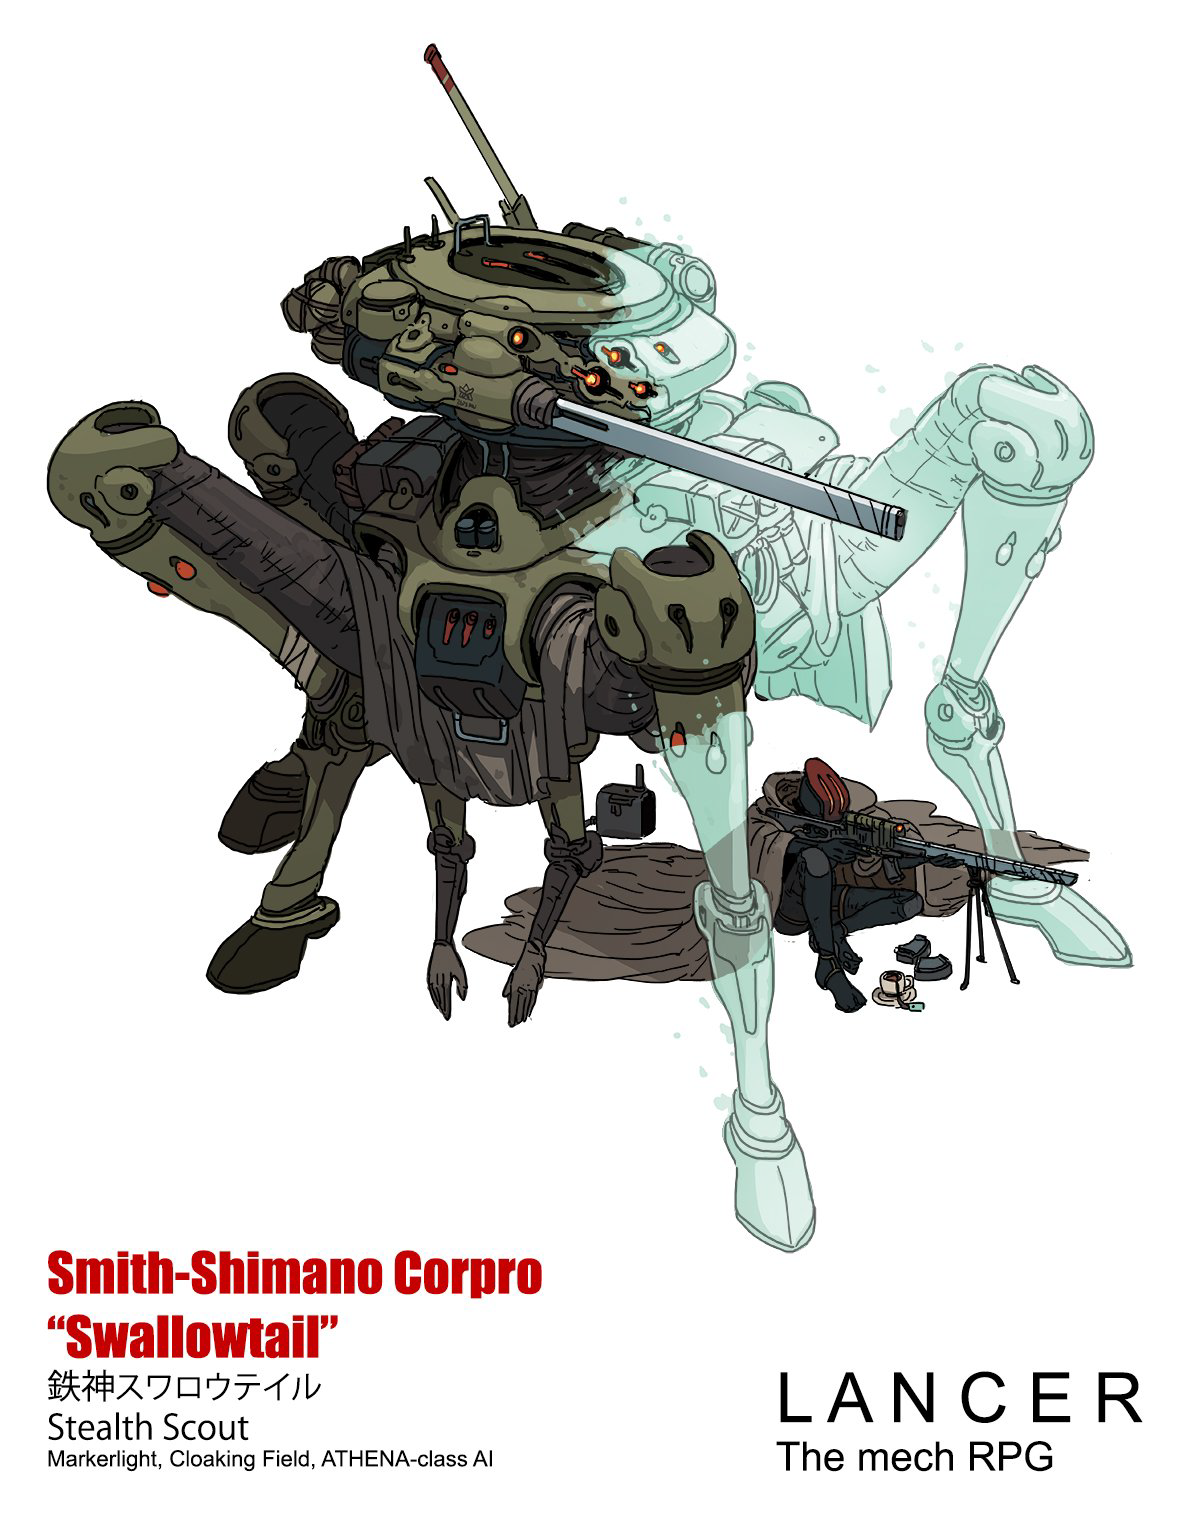
\includegraphics{Swallowtail}


                                          SSC SWALLOWTAIL

The SWALLOWTAIL platform is Smith-Shimano’s primary long range/long term scouting platform,
built for rapid and sustained ranging across hostile, volatile environments.

                                                     License:





I. Markerlight, Scout Drone Nexus

II. SWALLOWTAIL FRAME,  Oracle light machine gun, Low Profile

III. ATHENA-class NHP, Cloaking Field


                                                SWALLOWTAIL

  HP: 6           Evasion: 10                            Speed: 6            Heat Cap: 6         Sensors: 20

  Armor: 0        E-Defense: 10                          Size: 1             Repair Cap: 3       Tech Attack:
                                                                                                 +1

                                                      TRAITS:

  Integrated Cloak: If the Swallowtail doesn’t move during its turn, it becomes invisible at the end of its
  turn. This invisibility immediately breaks if it moves, attacks, takes a reaction, or starts its next turn.

  Prophetic Scanners: Targets suffering from Lock On from the swallowtail are also Shredded

                                               SYSTEM POINTS: 6

                                                     MOUNTS:

  Aux/Aux                                                 Flex Mount

                                                   CORE system

                                          Cloudscout TACSIM Swarms

  Cloudscout TACSIM Swarms are packets of networked microsensors, launched in nonlethal mortar
  canisters that detonate high above the battlefield. Once seeded in such a way, the TACSIM program the
  cloudscouts create begin to run brevity cycles: tight, contained simulations of tactical possibility.
  Probability results are then fed to the pilot’s NHP, who in turn feeds it to the pilot and their networked
  squad members, ensuring high-probability successful outcomes.

  Active (Requires 1 core power): Prophetic Interjection
  Until the end of the current challenge, once per round, as a reaction when an allied target you can see
  is damaged by another target you can see, you can make a systems check. On success, the attack
  hitting was actually a simulation that your mech predicted. Your ally gains resistance to all the damage
  from that attack, and your ally can move 3 in any direction to where they ‘actually’ were. This
  movement does not provoke reactions and ignores engagement.

Scout Drone Nexus
The scout drone is a small, active-camouflaged mini-drone launched from a mounted LOTUS projector.

The LOTUS projector fires scout drones at subsonic speeds in bursts of ten, blanketing a wide area with
the single-use drones in order to relay information about terrain and targets within.

2 SP

Drone, Quick Action





Sensor Range

When you use this system, you can deploy your drone to an area in sensor range and line of
sight. The drone then emits a burst 2 area around it that grants the following benefits:

  - Gain perfect vision of that area

  - Hostile targets that end their turn in the area immediately lose invisibility or hiding.

  - Reveal current HP, Evasion, E-defense, and heat levels of targets in that area

The drone can be attacked and targeted as normal, but it is also permanently invisible. It can be
recalled or redeployed by taking this action again.


Markerlight
Main Rifle

1 SP

Range 20


This weapon deals no damage and cannot deal damage (from talents or otherwise) or take
weapon mods, but on hit, it inflicts Lock On on your target at the end of your turn.


ORACLE Light machine gun
Auxiliary Rifle

1 SP, Arcing, Accurate

Range 15

1d3 kinetic damage


Low Profile

A hallmark of a well thought out mech platform is the ability for pilots to work with their technicians to

adapt their stock model to the specifications of the environments they operate in. Lowering a mech’s profile
removes extraneous protrusions, tunes any broadcast software, and masks heat signatures — all an effort
to reduce optical and scanner signatures.

1 SP, Unique
Protocol
Your mech can retract its major systems to reduce its profile. You can activate this protocol at
the start of your turn. While active:

     -   Rolls to find your mech while hidden are made at +1 Difficulty

     -   All ranged and tech attacks against you are made at +1 Difficulty

     -   Your mech is Slowed and cannot make ranged, melee, or tech attacks


ATHENA-class NHP

Smith-Shimano’s ATHENA is the pinnacle of total hyperspectral environmental facsimile. Through a

combination of unfettered Omninet access, hyperspectral relays fired out from a Cloudscout TACSIM
projector, sub-networked squadmates, and active/hostile intrusion protocols, ATHENA bootstraps a near-
flawless reconstruction of the immediate environment around its host core. ATHENA is unparalleled in its

processing power, and with this reconstructed environment it can provide trustworthy, accurate advising to
pilots in need of strategic counsel.
ATHENA clones tend to be patient, cautious, and measured in their relations with their pilots.





3 SP, Unique

AI

Your mech gains the AI property and gains the ATHENA protocol:


         ATHENA protocol
          Quick Action

          Choose a blast 3 area within 1 mile of you. Your AI constructs a perfect, real-time, 3d
          model of this are that you can rotate and interact with, including actors that move in and
          out of that area, and extreme detail. You can re-target or move this area by taking this
          quick action again. It lasts until the end of the current scene (or about 10 minutes in
          narrative time).


         Your mech gains perfect vision of this area and can relay this to allies, letting any attacks
         from yourself or allies in the area ignore cover. Hostile targets that end their turn in this
          area lose invisibility or hiding, and you can see the current heat and HP levels of all
         targets in the area.


Cloaking Field

SSC’s milspec cloaking field is the result of extensive experimentation in cooling and light-reflecting
technology. Born from a need to bounce harmful radiation away from ships and EVA modules in deep

space, the SSC-MILSPEC LIGHTBEND/OVERCLOAK is a system often equipped by ranger and long-patrol
scout pilots to ensure not only radiation protection, but optical concealment as well. The light and
radiation-bending properties of the LB/OC conceals anything inside of its projected bubble from sensor

suites and optical spotting.

4 SP

2 heat (self)
Quick Action

You can activate or deactivate the light bending properties of this module as a quick action. It
lasts until the end your next turn. When you activate this module, your mech and all allied targets
within a burst 3 area centered on you become invisible while they remain in the area. This area
moves when you move, and remains centered on you. If you become stunned, shut down, or
take damage, this module immediately becomes inactive.
